\documentclass[letterpaper,10pt]{article}

\usepackage{enumitem}
\usepackage{titling}
\usepackage{listings,listings-rust}
\usepackage{url}
\usepackage{soul}
\usepackage{hyperref}
\usepackage{setspace}
\usepackage{subfig}
\usepackage{sectsty}
\usepackage{pdfpages}
\usepackage{colortbl}
\usepackage{multirow}
\usepackage{multicol}
\usepackage{relsize}
\usepackage{amsmath}
\usepackage{wasysym}
\usepackage{fancyvrb}
\usepackage[yyyymmdd]{datetime}
\usepackage{amsmath,amssymb,amsthm,graphicx,xspace}
\usepackage[titlenotnumbered,noend,noline]{algorithm2e}
\usepackage[compact]{titlesec}
\usepackage{XCharter}
\usepackage[T1]{fontenc}
\usepackage[scaled]{beramono}
\usepackage[normalem]{ulem}
\usepackage{booktabs}
\usepackage{tikz}
\usetikzlibrary{arrows.meta,automata,shapes,trees,matrix,chains,scopes,positioning,calc,decorations.pathreplacing}
\tikzstyle{block} = [rectangle, draw, fill=blue!20, 
    text width=2.5em, text centered, rounded corners, minimum height=2em]
\tikzstyle{bw} = [rectangle, draw, fill=blue!20, 
    text width=4em, text centered, rounded corners, minimum height=2em]

\definecolor{namerow}{cmyk}{.40,.40,.40,.40}
\definecolor{namecol}{cmyk}{.40,.40,.40,.40}
\renewcommand{\dateseparator}{-}

\let\LaTeXtitle\title
\renewcommand{\title}[1]{\LaTeXtitle{\textsf{#1}}}

\lstset{basicstyle=\footnotesize\ttfamily,breaklines=true}

\newcommand{\CPP}{C\nolinebreak\hspace{-.05em}\raisebox{.4ex}{\tiny\bf +}\nolinebreak\hspace{-.10em}\raisebox{.4ex}{\tiny\bf +}}
\def\CPP{{C\nolinebreak[4]\hspace{-.05em}\raisebox{.4ex}{\tiny\bf ++}}}

\newcommand{\handout}[5]{
  \noindent
  \begin{center}
  \framebox{
    \vbox{
      \hbox to 5.78in { {\bf ECE459: Programming for Performance } \hfill #2 }
      \vspace{4mm}
      \hbox to 5.78in { {\Large \hfill #4  \hfill} }
      \vspace{2mm}
      \hbox to 5.78in { {\em #3 \hfill \today} }
    }
  }
  \end{center}
  \vspace*{4mm}
}

\newcommand{\lecture}[3]{\handout{#1}{#2}{#3}{Lecture#1}}
\newcommand{\tuple}[1]{\ensuremath{\left\langle #1 \right\rangle}\xspace}

\addtolength{\oddsidemargin}{-1.000in}
\addtolength{\evensidemargin}{-0.500in}
\addtolength{\textwidth}{2.0in}
\addtolength{\topmargin}{-1.000in}
\addtolength{\textheight}{1.75in}
\addtolength{\parskip}{\baselineskip}
\setlength{\parindent}{0in}
\renewcommand{\baselinestretch}{1.5}
\newcommand{\term}{Winter 2020}

\singlespace


\begin{document}

\lecture{ 34 --- DevOps for P4P }{\term}{Patrick Lam \& Jeff Zarnett}

\section*{DevOps for P4P}
So far, we've talked almost exclusively about one-off computations:
you want to figure out the answer to a question, and you write code to
do that. Our assignments have been like that, for instance. There are lots
of programs in the world at are solely on-demand. Still, a lot
of the time we want to keep systems running over time. That is, a service
that is available (if not always then close to it) and responds to requests
whenever they may happen to arrive. That gets us
into the notion of operations. Your service or product is more likely than 
ever to have at least some component that's server side (whether hosted
in a cloud service or not) that's under your control.

The theme today will be using software development skills in
operations (e.g., system administration, database management, etc). This
does have some relevance, because the operations (or IT, if you prefer)
processes and procedures, while different from development, have some
similarities. 

Even when we've talked about multi-computer tools like cloud
computing, it still has not been in the context of keeping your
systems operational over longer timescales. The trend today is away
from strict separation between a development team, which writes the
software, and an operations team, which runs the software.

\begin{center}
	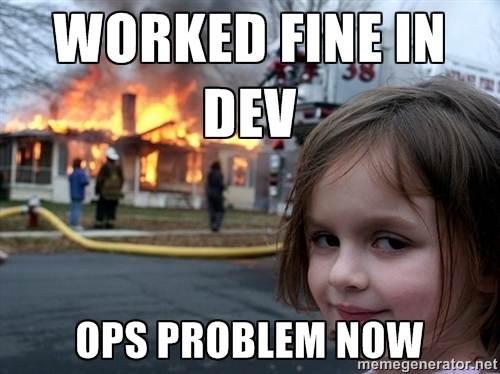
\includegraphics[width=0.45\textwidth]{images/devops.jpg}
\end{center}

The separation is totally nonexistent at the typical startup company. There isn't the money to pay for separate developers and operations teams. And in the beginning there's probably not that many servers, just a few demo systems, test systems, etc... but it spirals out from there. You're not really going to ask the sales team to manage these servers, are you? So, there's DevOps. 

Is DevOps a good idea? Like most ideas it can be used for both good and evil. There's a lot to be said for letting the developers be involved in all the parts of the software from development to deployment to management to training the customers. Developers can learn a lot by having to do these kinds of things, and be motivated to make proper management and maintenance tools and procedures. If we make the pain of operations felt by developers, they might do something about it. If it's the problem of another team, somehow those tickets just never make it to the top of the backlog.

Thanks to Chris Jones and Niall Murphy for the following points.

\subsection*{Configuration as code}
Systems have long come with complicated configuration options.
Sendmail is particularly notorious, but apache and nginx aren't super
easy to configure either.\footnote{If anyone should be foolish enough to want to look into procmail, well, good luck to you...} The first principle is to treat \emph{configuration as code}. 
Therefore:
\begin{itemize}
\item use version control on your configuration.
\item implement code reviews on changes to the configuration.
\item test your configurations: that means that you check that they
  generate expected files, or that they spawn expected
  services. (Behaviours, or outcomes.) Also, configurations should
  ``converge''. Unlike code, they might not terminate; we're talking
  indefinitely-running services, after all. But the CPU usage should
  go down after a while, for instance.
\item aim for a suite of modular services that integrate together smoothly.
\item refactor configuration files (Puppet manifests, Chef recipes, etc);
\item use continuous builds (more on that later).
\end{itemize}

Furthermore, it's an excellent idea to have tools for configuration. It's not enough to just have a wiki page or github document titled ``How to Install AwesomeApp'' (fill in name of program here). Complicated means mistakes and people will forget steps. Don't let them make mistakes: make it automatic.

One particular example of applying all those principles to infrastructure
is Terraform. Its whole purpose is to manage your config as codes
situation where you want to run your code using a cloud provider (e.g., AWS), 
then you can control the infrastructure using Terraform: you write the
configuration files that say you want this service with these permissions
(and any other details) and then you can apply that configuration easily.
Terraform does support a ``plan'' operation so it can tell you what it will
do, so you can verify that, before anything is actually changed. Then, if 
you are happy with it, apply it! 

\paragraph{Containers.} What about containers? Well, let's see how we got there first. In the beginning, you had services where you installed the binaries and config files by hand. That sucked. So there were packages; a package includes everything the program needs (including a list of dependencies) and a script to install it and set it up. Great! But if you just install multiple services on the same machine you don't get isolation and you might have incompatible versions of dependencies and you're in RPM hell (see also: JAR hell, classloader hell, and DLL hell).

Right, so instead you say you should have virtual machines: you configure the VM parameters and install the guest OS and set it up (and you can copy-paste the initial image, which helps) but for every application you have a guest operating system running underneath. Maybe we don't need every app to have its own guest OS; why do we have to install the same security patch ten times...?

Containerization gives many of the advantages of this separation, but without nearly so much overhead of the guest operating systems (both its maintenance and runtime costs). Containers are run by a container engine so there is some abstraction of the underlying hardware, and the container is assembled from a specification that says what libraries, tools, etc. are needed. And thus when the container is built and deployed it is sufficiently isolated but shares (in read only mode) where it can. So a container is a very lightweight VM, in some sense. See this diagram from~\cite{netappcontainer}:

\begin{center}
	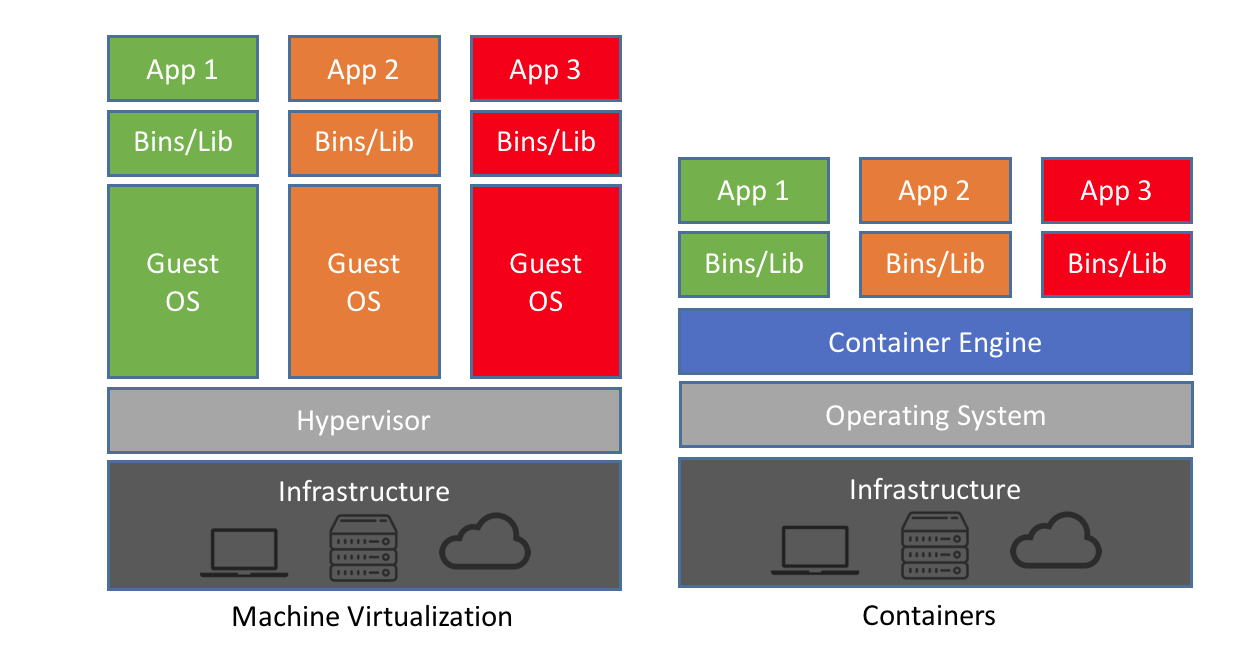
\includegraphics[width=0.55\textwidth]{images/cvm.png}
\end{center}

Containers do potentially come with a downside of letting you just not upgrade things. Whereas before if you installed the OS patches you might get updates in your shared libraries, the container allows you to keep an old insecure version of a library around forever. So, don't do that. Keeping on top of security updates is important. Let's talk about that, actually.

\paragraph{Security, report to the bridge.}
Having an always-available service accessible over the internet makes security a very big concern. You can run some program with tons of security vulnerabilities offline and feel that the security problems can be managed, but when it's online the risk is enormous. All kinds of vulnerabilities are a problem, but I'll call out two of them as being especially bad: code execution/injection and data leakage (information exposure). 

Code execution is exactly what it sounds like: attackers run their code using your platform. They can mess with your data, send spam or harrassing e-mails to your customers, take services without paying for them, mine bitcoin at your expense, and many other things. Sometimes these are company-ending events.

Information exposure is not only terrible for your company's reputation, but also against privacy laws and data protection regulations. A breach of the EU GDPR can get very expensive. See \url{https://www.enforcementtracker.com/} to find out which companies have recently gotten their wrists slapped or a huge fine. At the time of writing, the record holder is Marriott International Inc of the UK with a fine of 	110,390,200 EUR which is roughly 171,898,556.93 CAD (using exchange rates from October 2020). Not exactly pocket change.

There are some companies out there that will check your code for libraries with versions having known security vulnerabilities. This is transitive, so if your app depends on some library that depends on a parsing library with a vulnerability, the vulnerability is noticed and reported. Each vulnerability is usually assigned a severity and the service may even suggest that updating from version X to Y will solve the problem. They can say this because they observe that a vulnerability reported in version X of a library is reported as fixed in version Y. 

Sadly, when there is an updated version of a library, there may be breaking changes in it, so an upgrade might be more painful than just changing a version number and rebuilding. It may also take time for libraries to correct and release a fixed version of the library. In the meantime, you may need to implement some mitigation of your own, or just keep an eye open for when the patch is released. These mean that the vulnerability checks give you the ability to ignore or snooze the alert. Tempting as it is to do that and get on with other work, it's leaving the vulnerability in your code. Good practice would be for reviewers to discourage ignoring if it can be avoided.

As with the other parts of managing your application, like build and deployment, checking for vulnerabilities should be an automatic process as part of your build and release procedures. 

\subsection*{Servers as cattle, not pets}
By servers, I mean servers, or virtual machines, or containers. It's much better to have a reproducible process for deployment of a server than doing it manually every single time. The amount of manual intervention should be minimized and ideally zero. If this is done you can save a lot of hours of time, reduce errors, and allow for automatic scaling (starting and stopping servers depending on demand).

The title references the idea that cattle are dealt with as a herd: you try to get the whole group to move along and do what they need. Pets are individuals, though, and you'll treat them all differently. This amount of individual attention quickly becomes unmanageable and there's no reason why you should worry about these differences in a world with virtualization (containers) or similar. 

As with managing infrastructure, I'll give a specific example: Kubernetes. This is used to automate deploying and scaling of applications. This means you don' have to manually manage them; if you want to deploy a new version of a container, just tell Kubernetes to do it. The part about how it does so is that it provides a framework for your environment. It can do load balancing, automatic rollouts and reverts (if something went wrong), will figure out what instances run on what hardware, check the health of instances, replace them if they die, and more.

subsection*{Common infrastructure}
Use APIs to access your infrastructure. That is, you should view different parts of your infrastructure as having an interface and communication is done exclusively via the interface/API. This reduces the coupling between different components, and, as we've discussed, allows you to scale the parts that need scaling. 

Try to avoid not-invented-here syndrome: it is usually better to use an open-source tool (or a commercial one) than to roll your own. Some examples might be:
\begin{itemize}
\item storage: some sort of access layer (e.g., MongoDB or S3);
\item naming and discovery infrastructure (e.g., Consul) (more below);
\item monitoring infrastructure (e.g., Prometheus).
\end{itemize}

However, be prepared to build your own tools if needed. Sometimes what you want, or need, doesn't exist (yet). Think carefully about whether this service that is needed is really part of your core competence and whether creating it adds sufficient value to the business. It's fun to make your own system and all, but are you doing what you're best at? 

Think extra carefully if you plan to do roll your own anything that is security or encryption related. I'm just going to say that unless you have experts on staff who know the subject really well and you're willing to pay for external audits and the like, you're more likely to end up with a terrible security breach than a terrific secure system. 

As a second followup soapbox point to that: if what you are looking for doesn't exist, there might be a reason, Maybe the reason is that you are the first to think of it, but consider the possibility that it's not that good of an idea (either due to inefficiency or just not being great in principle).  

\subsection*{Naming}
Naming is one of the hard problems in computing. There is a saying that there are only two hard things in computers: cache invalidation, naming things, and off by one errors.  There are a
lot of ways to name things. We'll talk about
systems/VMs\footnote{\url{http://mnx.io/blog/a-proper-naming-scheme}},
but naming is necessary for resources of all kinds.

In brief:
\begin{itemize}
\item use canonical one-word names for servers;
\item but, use aliases to specify functions, e.g. 1) geography (nyc); 2) environment (dev/tst/stg/prod); 
3) purpose (app/sql/etc); and 4) serial number.
\end{itemize}
This enables you to have a way of referring to each machine in an absolute sense, but also 
allows you to use functional names when creating dependencies between systems.

There's also the Java package approach of infinite dots: live.application.customer.webdomain.com or however you want to call it. But pick something and be consistent.

\subsection*{Other Topics}
Beyond the five principles above, there are a couple more techniques that particularly apply to
DevOps:

\paragraph{Continuous Integration.} 
This is now a best practice. It's enabled by the use of version control, good tests, and scripted deployments.
It works like this:
\begin{itemize}
\item pull code from version control;
\item build;
\item run tests;
\item report results.
\end{itemize}
What's also key is a social convention to not break the build. These things get done automatically on every commit and the results are sent to people by e-mail or instant messenger (because e-mail is for old people, right?).\footnote{I did work at a company where the person who broke the build got a sign outside his cubicle that said IOTD - Idiot of the Day. I'm not too proud to admit that I won this award on my last day of the co-op term.}

%https://jenkins-ci.org/sites/default/files/jenkins_logo.png

CI is good for all code, but it's especially good for configuration-as-code, which is especially likely
to break in different environments.

\paragraph{Canarying.}
%http://www.post-gazette.com/image/2013/10/29/ca27,76,1566,1822/Canary.jpg
Deploy new software incrementally alongside production software, also known as ``test in prod''. Sometimes
you just don't know how code is really going to work until you try it. After, of course, you use your best
efforts to make sure the code is good. Steps:
\begin{itemize}
\item stage for deployment;
\item remove canary servers from service;
\item upgrade canary servers;
\item run automatic tests on upgraded canaries;
\item reintroduce canary servers into service;
\item see how it goes!
\end{itemize}
Of course, you should implement your system so that rollback is possible.

\paragraph{Monitoring.}

Monitoring is surprisingly difficult. There are a lot of recommendations about what to monitor and what to do about it. We care about performance so here are a few things to think about:

\begin{itemize}
	\item CPU Load
	\item Memory Utilization
	\item Disk Space
	\item Disk I/O
	\item Network Traffic
	\item Clock Skew
	\item Application Response Times
\end{itemize}

With multiple systems, you will want some sort of dashboard that gives an overview of all the multiple systems in a summary. The summary needs to be sufficiently detailed that you can detect if anything is wrong, but not an overwhelming wall of data. Then you do not necessarily want to pay someone to stare at the dashboard and press the  ``Red Alert!'' button if anything goes out of some preset range of what is okay. No, for that we need some automatic monitoring.

Here's one way to think about it. 
% track down the source here: Niall Murphy interview.
\begin{itemize}
\item {\bf Alerts}: a human must take action now;
\item {\bf Tickets}: a human must take action soon (hours or days);
\item {\bf Logging}: no need to look at this except for forensic/diagnostic purposes.
\end{itemize}
A common bad situation is logs-as-tickets: you should never be in the
situation where you routinely have to look through logs to find
errors. Write code to scan logs.

It is very important to be judicious about the use of alerts. If your alerts are too common, they get ignored. When you hear the fire alarm in a building, chances are your thought is not ``the building is on fire; I should leave it immediately in an orderly fashion.''. More likely your reaction is ``great, some jerk\footnote{This is the PG-13 version of what I actually think.} has pulled the fire alarm for a stupid prank or to get out of failing a midterm.'' This is because we have been trained by far too many false alarms to think that any alarm is a false one. It's a good heuristic; you'll be correct most of the time. But if there is an actual fire, you will not only be wrong, you might also be dead.

Still, alerts and tickets are a great way to make user pain into developer pain. Being woken up in the middle of the night (... day? A lot of programmers are nocturnal, now that I think of it) because of some SUPER CRITICAL ticket OMG KITTENS ARE ENDANGERED is an excellent way to learn the lesson that production code needs to be written carefully, reviewed, QA'd, and perhaps run by a customer or two before it gets deployed to everyone. Developers, being human (... grant me some leeway here), will probably take steps to avoid their pain\footnote{There is a great quotation to this effect by Fr\'ed\'eric Bastiat about how men will avoid pain and work is pain.}. and they will take steps that keep these things from happening in the future: good processes and monitoring and all that goes with it.


\bibliographystyle{alphaurl}
\bibliography{459}


\end{document}
